\documentclass[a4paper, final]{article}
\usepackage{cmap}
%\usepackage{literat} % Нормальные шрифты
\usepackage[14pt]{extsizes} % для того чтобы задать нестандартный 14-ый размер шрифта
\usepackage[T2A]{fontenc}
\usepackage[UTF8]{inputenc}
\usepackage[russian]{babel}
\usepackage{listings} %листинги
\usepackage{amsmath}
\usepackage{amssymb} % Для красивого значка пустого множества
\usepackage[left=25mm, top=20mm, right=20mm, bottom=20mm, footskip=10mm]{geometry}
\usepackage{ragged2e} %для растягивания по ширине
\usepackage{setspace} %для межстрочного интервала
\usepackage{indentfirst} % для абзацного отступа
\usepackage{moreverb} %для печати в листинге исходного кода программ
\renewcommand\verbatimtabsize{4\relax}
\renewcommand\listingoffset{0.2em} %отступ от номеров строк в листинге
\renewcommand{\arraystretch}{1.4} % изменяю высоту строки в таблице
\usepackage[font=small, singlelinecheck=false, justification=centering, format=plain, labelsep=period]{caption} %для настройки заголовка таблицы
\usepackage{listingsutf8}
\usepackage{xcolor} % цвета
\usepackage{hyperref}% для гиперссылок
\usepackage{enumitem} %для перечислений
\usepackage{titlesec}
\usepackage{graphicx}
\graphicspath{ {./Рисунки/} }
%\usepackage{float}
\usepackage{booktabs}
\usepackage{floatrow}
\usepackage[final]{pdfpages}
\usepackage{multirow}
\usepackage{array}
\usepackage{tabularx}
\usepackage{subfigure}

\definecolor{apricot}{HTML}{FFF0DA}
\definecolor{mygreen}{rgb}{0,0.6,0}
\definecolor{string}{HTML}{B40000} % цвет строк в коде
\definecolor{comment}{HTML}{008000} % цвет комментариев в коде
\definecolor{keyword}{HTML}{1A00FF} % цвет ключевых слов в коде
\definecolor{morecomment}{HTML}{8000FF} % цвет include и других элементов в коде
\definecolor{captiontext}{HTML}{FFFFFF} % цвет текста заголовка в коде
\definecolor{captionbk}{HTML}{999999} % цвет фона заголовка в коде
\definecolor{bk}{HTML}{FFFFFF} % цвет фона в коде
\definecolor{frame}{HTML}{999999} % цвет рамки в коде
\definecolor{brackets}{HTML}{B40000} % цвет скобок в коде


% Выравнивание подписи влево для таблиц
\captionsetup[table]{justification=raggedright, singlelinecheck=false}


\AtBeginDocument{\renewcommand{\contentsname}{Содержание}}
\AtBeginDocument{\renewcommand{\refname}{Список источников}}
% Настраиваем листинги, чтобы они использовали счётчик figure
\AtBeginDocument{
  \renewcommand{\thelstlisting}{\thefigure}  % Листинги используют тот же счетчик, что и рисунки
  \renewcommand{\lstlistingname}{Рис.}    % Меняем подпись
}

% Автоматически увеличиваем счетчик figure перед каждым листингом
\let\oldlstlisting\lstlisting
\renewcommand{\lstlisting}[1][]{%
    \refstepcounter{figure}% Увеличиваем счетчик figure
    \oldlstlisting[#1]% Вызываем оригинальную команду lstlisting
}
\lstset{
    captionpos=b
}
\newcommand{\specialcell}[2][l]{\begin{tabular}[#1]{@{}l@{}}#2\end{tabular}} % Алиас для таблиц

\floatsetup[table]{style=plain,capposition=top} % Подпись таблицы сверху
\setlist[enumerate,itemize]{leftmargin=1.2cm} %отступ в перечислениях

\hypersetup{colorlinks,
  allcolors=[RGB]{010 090 200}} %красивые гиперссылки (не красные)

% подгружаемые языки - подробнее в документации listings (это всё для листингов)
\lstloadlanguages{ [LaTeX] TeX}
% включаем кириллицу и добавляем кое−какие опции
\lstset{language =[LaTeX] TeX, % выбираем язык по умолчанию
extendedchars=true , % включаем не латиницу
escapechar = | , % |«выпадаем» в LATEX|
frame=tb , % рамка сверху и снизу
commentstyle=\itshape , % шрифт для комментариев
stringstyle =\bfseries} % шрифт для строк

\textheight=24cm % высота текста
\textwidth=16cm % ширина текста
\oddsidemargin=0pt % отступ от левого края
\topmargin=-1.5cm % отступ от верхнего края
\parindent=24pt % абзацный отступ
\parskip=0pt % интервал между абзацами
\tolerance=2000 % терпимость к "жидким" строкам
\flushbottom % выравнивание высоты страниц

\begin{document} % начало документа
\setcounter{tocdepth}{2} % Вложенность не больше 2 в содержании
\lstset{
  language=haskell, % Язык кода по умолчанию
  morekeywords={*,...}, % если хотите добавить ключевые слова, то добавляйте
  % Цвета
  keywordstyle=\color{keyword}\ttfamily\bfseries,
  %stringstyle=\color{string}\ttfamily,
  stringstyle=\ttfamily\color{red!50!brown},
  commentstyle=\color{comment}\ttfamily,
  morecomment=[l][\color{morecomment}]{\#},
  % Настройки отображения
  breaklines=true, % Перенос длинных строк
  basicstyle=\ttfamily\footnotesize, % Шрифт для отображения кода
  backgroundcolor=\color{bk}, % Цвет фона кода
  frame=single,xleftmargin=\fboxsep,xrightmargin=-\fboxsep, % Рамка, подогнанная к заголовку
  rulecolor=\color{frame}, % Цвет рамки
  tabsize=3, % Размер табуляции в пробелах
  % Настройка отображения номеров строк. Если не нужно, то удалите весь блок
  numbers=left, % Слева отображаются номера строк
  stepnumber=1, % Каждую строку нумеровать
  numbersep=5pt, % Отступ от кода
  numberstyle=\small\color{black}, % Стиль написания номеров строк
  % Для отображения русского языка
  extendedchars=true,
  literate={Ö}{ {\"O} }1
  {~}{ {\textasciitilde} }1
  {а}{ {\selectfont\char224} }1
  {б}{ {\selectfont\char225} }1
  {в}{ {\selectfont\char226} }1
  {г}{ {\selectfont\char227} }1
  {д}{ {\selectfont\char228} }1
  {е}{ {\selectfont\char229} }1
  {ё}{ {\"e} }1
  {ж}{ {\selectfont\char230} }1
  {з}{ {\selectfont\char231} }1
  {и}{ {\selectfont\char232} }1
  {й}{ {\selectfont\char233} }1
  {к}{ {\selectfont\char234} }1
  {л}{ {\selectfont\char235} }1
  {м}{ {\selectfont\char236} }1
  {н}{ {\selectfont\char237} }1
  {о}{ {\selectfont\char238} }1
  {п}{ {\selectfont\char239} }1
  {р}{ {\selectfont\char240} }1
  {с}{ {\selectfont\char241} }1
  {т}{ {\selectfont\char242} }1
  {у}{ {\selectfont\char243} }1
  {ф}{ {\selectfont\char244} }1
  {х}{ {\selectfont\char245} }1
  {ц}{ {\selectfont\char246} }1
  {ч}{ {\selectfont\char247} }1
  {ш}{ {\selectfont\char248} }1
  {щ}{ {\selectfont\char249} }1
  {ъ}{ {\selectfont\char250} }1
  {ы}{ {\selectfont\char251} }1
  {ь}{ {\selectfont\char252} }1
  {э}{ {\selectfont\char253} }1
  {ю}{ {\selectfont\char254} }1
  {я}{ {\selectfont\char255} }1
  {А}{ {\selectfont\char192} }1
  {Б}{ {\selectfont\char193} }1
  {В}{ {\selectfont\char194} }1
  {Г}{ {\selectfont\char195} }1
  {Д}{ {\selectfont\char196} }1
  {Е}{ {\selectfont\char197} }1
  {Ё}{ {\"E} }1
  {Ж}{ {\selectfont\char198} }1
  {З}{ {\selectfont\char199} }1
  {И}{ {\selectfont\char200} }1
  {Й}{ {\selectfont\char201} }1
  {К}{ {\selectfont\char202} }1
  {Л}{ {\selectfont\char203} }1
  {М}{ {\selectfont\char204} }1
  {Н}{ {\selectfont\char205} }1
  {О}{ {\selectfont\char206} }1
  {П}{ {\selectfont\char207} }1
  {Р}{ {\selectfont\char208} }1
  {С}{ {\selectfont\char209} }1
  {Т}{ {\selectfont\char210} }1
  {У}{ {\selectfont\char211} }1
  {Ф}{ {\selectfont\char212} }1
  {Х}{ {\selectfont\char213} }1
  {Ц}{ {\selectfont\char214} }1
  {Ч}{ {\selectfont\char215} }1
  {Ш}{ {\selectfont\char216} }1
  {Щ}{ {\selectfont\char217} }1
  {Ъ}{ {\selectfont\char218} }1
  {Ы}{ {\selectfont\char219} }1
  {Ь}{ {\selectfont\char220} }1
  {Э}{ {\selectfont\char221} }1
  {Ю}{ {\selectfont\char222} }1
  {Я}{ {\selectfont\char223} }1
  {\{}{ { {\color{brackets}\{} } }1 % Цвет скобок {
  {\} }{ { {\color{brackets}\} } } }1 % Цвет скобок }
}

% НАЧАЛО ТИТУЛЬНОГО ЛИСТА
\begin{center}
\hfill \break
\hfill \break
\normalsize{МИНИСТЕРСТВО НАУКИ И ВЫСШЕГО ОБРАЗОВАНИЯ РОССИЙСКОЙ ФЕДЕРАЦИИ\\
 федеральное государственное автономное образовательное учреждение высшего образования «Санкт-Петербургский политехнический университет Петра Великого»\\[5pt]}
\normalsize{Институт компьютерных наук и кибербезопасности}\\[5pt] 
\normalsize{Высшая школа технологий искусственного интеллекта}\\[5pt] 
\normalsize{Направление: 02.03.01 Математика и компьютерные науки}\\

\hfill \break
\hfill \break
\hfill \break
\large{Теория алгоритмов}\\
\hfill \break
\large{Отчёт по выполнению курсовой работы}\\
\large{\textit{<<Синтез функциональной схемы электронных часов>>\\}}
\large{Вариант 11\\}

\hfill \break
\hfill \break
\end{center}
 
\small{ 
\begin{tabular}{lrrl}
\!\!\!Студент, & \hspace{2cm} & & \\
\!\!\!группы 5130201/20102 & \hspace{2cm} & \underline{\hspace{3cm}} &Гаар В.С. \\\\
\!\!\!Преподаватель & \hspace{2cm} & \underline{\hspace{3cm}} &  Востров А.В. \\\\
&&\hspace{5cm}
\end{tabular}
\begin{flushright}
\hfill \break
<<\underline{\hspace{1cm}}>>\underline{\hspace{2.5cm}} 2024 г.
\end{flushright}
}

\hfill \break
\hfill \break
\begin{center} \small{Санкт-Петербург, 2024} \end{center}
\thispagestyle{empty} % выключаем отображение номера для этой страницы

% КОНЕЦ ТИТУЛЬНОГО ЛИСТА
\newpage

\tableofcontents

\newpage

\cleardoublepage
\phantomsection
\addcontentsline{toc}{section}{Введение}
\section*{Введение}
Данный отчёт содержит в себе информацию о курсовой работе, в ходе выполнения которой было необходимо разработать функциональную схему электронных часов с заданными дополнительными функциями.

На функциональной схеме изображают функциональные части изделия (элементы, устройства и функциональные группы), участвующие в процессе, иллюстрируемом схемой, и связи между этими частями. Графическое построение схемы должно давать наиболее наглядное представление о последовательности процессов, иллюстрируемых схемой.

\newpage
\section{Постановка задачи}
Построить функциональную схему электронных часов, которые кроме отображения и корректировки времени (минут и часов) выполняют следующие функции, определённые вариантом 2101100:
\begin{itemize}
  \item А=2: отображают и позволяют корректировать день недели;
  \item B=1: режим работы часов 24-х часовой;
  \item C=0: отключение индикаторов с целью экономии электроэнергии отсутствует; 
  \item D=1: останов часов по нажатию кнопки;
  \item E=1: присутствует простой секундомер (сброс - запуск - останов);
  \item F=0: звуковая сигнализация отсутствует; 
  \item G=0: звуковой сигнал в устанавливаемое время (будильник) отсутствует.
\end{itemize}

\noindent Для построения управляющих воздействий было необходимо:
\begin{enumerate}
  \item Построить конечный автомат с состояниями системы часов.
  \item Построить и минимизировать функции импульсных и потенциальных команд.
  \item Построить функциональную схему часов с данными командами.
\end{enumerate}

\newpage
\section{Описание объекта управления}
Реализуемые электронные часы содержат индикаторную панель, показывающую время (часы, минуты) и день недели, и внешние кнопки управления a и b.

Для отображения времени используются:
\begin{enumerate}
  \item Шесть семисегментных дисплеев:
  \begin{itemize}
    \item старший десятичный разряд часов;
    \item младший десятичный разряд часов;
    \item старший десятичный разряд минут;
    \item младший десятичный разряд минут;
    \item первая буква аббревиатуры дня недели;
    \item вторая буква аббревиатуры дня недели.
  \end{itemize}
  
  \item Диод, отвечающий за режим работы часов: отображение времени часов/отображение времени секундомера.
\end{enumerate}

Для управления часами используются кнопки внешнего управления -- a и b. Входные воздействия на часы возможны нажатием одной из кнопок или их обеих одновременно.

\newpage
\section{Математическое описание}
\subsection{Модель конечного автомата}
Конечный автомат --- абстрактный автомат с конечным числом возможных внутренних состояний. 

Конечный автомат возможно формализовать как упорядоченную шестёрку: $M = (S, \Sigma, Y, s_0, \delta, \lambda)$, где
\begin{itemize}
  \item $S$ -- множество состояний конечного автомата;
  \item $\Sigma$ -- входной алфавит;
  \item $Y$ -- множество выходных сигналов;
  \item $s_0$ -- начальное состояние;
  \item $\delta : S \times \Sigma \rightarrow S$ -- функция переходов;
  \item $\lambda : S \times \Sigma \rightarrow Y$ -- функция выходов. 
\end{itemize}

Конечный автомат начинает работу в состоянии $s_0$, считывает входные воздействия и переходит в соответствующие функции переходов состояния, выводя соответствующие выходные данные.

\subsection{Реализация графа управляющего автомата}
Было выделено 7 состояний $S = \{S_0, S_1, S_2, S_3, S_4, S_5, S_6\}$, где
\begin{itemize}
  \item $S_0$ -- состояние отображения времени и дня недели (\textit{time}). В этом состоянии включены все индикаторы для отображения часов, минут и дня недели.
  \item $S_1$ -- состояние коррекции минут (\textit{minutes correction}). В этом состоянии горят только индикаторы минут.
  \item $S_2$ -- состояние коррекции часов (\textit{hours correction}). В этом состоянии горят только индикаторы часов.
  \item $S_3$ -- состояние коррекции дня недели (\textit{day of the week correction}). В этом состоянии горит только индикатор дня недели.
  \item $S_4$ -- состояние отображения времени секундомера (\textit{stopwatch}). На индикаторах -- идущее время (минуты и секунды) секундомера.
  \item $S_5$ -- состояние остановленного секундомера (\textit{stopwatch pause}). На индикаторах -- минуты и секунды секундомера. В этом состоянии секундомер не отсчитывает время.
  \item $S_6$ -- состояние остановленных часов (\textit{time stop}). На индикаторах -- часы, минуты и день недели. В этом состоянии время зафиксировано и не изменяется.
\end{itemize}

Множество выходных сигналов $Y = \{z_0, z_1, z_2, z_3, z_4, z_5, z_6\}$, где
\begin{itemize}
  \item $z_0$ -- нейтральный сигнал.
  \item $z_1$ -- прибавление единицы к минутам при корректировке;
  \item $z_2$ -- прибавление единицы к часам при корректировке;
  \item $z_3$ -- смена дня недели на следующий при корректировке;
  \item $z_4$ -- запуск секундомера;
  \item $z_5$ -- остановка/запуск секундомера;
  \item $z_6$ -- сброс текущего значения секундомера;
  \item $z_7$ -- остановка/запуск часов.
\end{itemize}

Входной алфавит $\Sigma = \{a, b, ab\}$, где
\begin{itemize}
  \item $a$ -- нажатие кнопки a;
  \item $b$ -- нажатие кнопки b;
  \item $ab$ -- нажатие обеих кнопок.
\end{itemize}

Начальное состояние $s_0$ автомата это состояние $S_0$ -- ''Отображение времени и дня недели''. 

Функция переходов и выходов представлены в Табл.~\ref{tbl:perehod_d} и Табл.~\ref{tbl:vihod_l} соответственно.

\begin{table}[h!]
    \centering
    \caption{Функция переходов $\delta$}
    \label{tbl:perehod_d}
    \footnotesize
    \begin{tabular}{|c|c|c|c|}
    \hline
          & \textbf{a} & \textbf{b} & \textbf{ab} \\
    \hline
    $\mathbf{S_0}$ & $S_1$ & $S_4$ & $S_6$ \\
    \hline
    $\mathbf{S_1}$ & $S_2$ & $S_1$ & $S_1$ \\
    \hline
    $\mathbf{S_2}$ & $S_3$ & $S_2$ & $S_2$ \\
    \hline
    $\mathbf{S_3}$ & $S_0$ & $S_3$ & $S_3$ \\
    \hline
    $\mathbf{S_4}$ & $S_4$ & $S_5$ & $S_0$ \\
    \hline
    $\mathbf{S_5}$ & $S_5$ & $S_4$ & $S_0$ \\
    \hline
    $\mathbf{S_6}$ & $S_6$ & $S_6$ & $S_0$\\
    \hline
    \end{tabular}
\end{table}

\begin{table}[h!]
  \centering
  \caption{Функция выходов $\lambda$}
  \label{tbl:vihod_l}
  \footnotesize
  \begin{tabular}{|c|c|c|c|}
  \hline
        & \textbf{a} & \textbf{b} & \textbf{ab} \\
  \hline
  $\mathbf{S_0}$ & $z_0$ & $z_0$ & $z_7$ \\
  \hline
  $\mathbf{S_1}$ & $z_0$ & $z_1$ & $z_0$ \\
  \hline
  $\mathbf{S_2}$ & $z_0$ & $z_2$ & $z_0$ \\
  \hline
  $\mathbf{S_3}$ & $z_0$ & $z_3$ & $z_0$ \\
  \hline
  $\mathbf{S_4}$ & $z_4$ & $z_5$ & $z_0$ \\
  \hline
  $\mathbf{S_5}$ & $z_6$ & $z_5$ & $z_0$ \\
  \hline
  $\mathbf{S_6}$ & $z_0$ & $z_0$ & $z_7$\\
  \hline
  \end{tabular}
\end{table}

\newpage
На Рис.~\ref{img:automaton} представлен реализованный конечный автомат.

\begin{figure}[H]
   \centering
   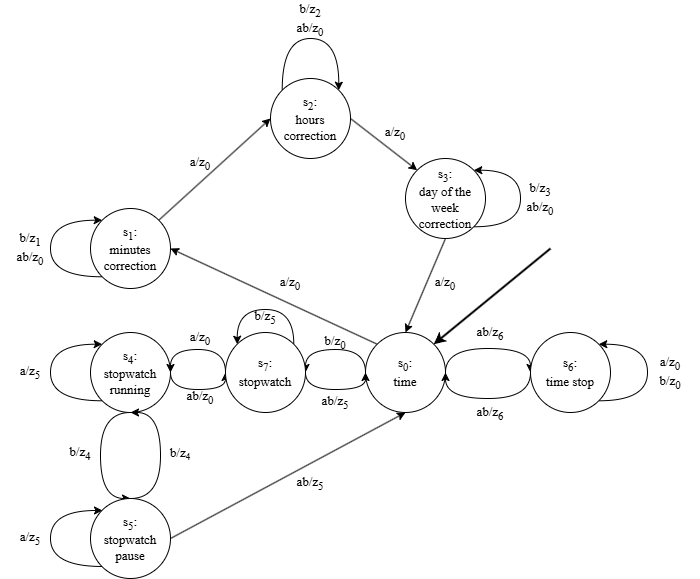
\includegraphics[width=\linewidth]{automaton.png}
   \caption{Конечный автомат}
   \label{img:automaton}
\end{figure}

Этому графу переходов соответствует следующая таблица переходов (Табл.~\ref{tbl:perehod}).

\newpage
\begin{table}[H]
  \centering
  \caption{Таблица переходов}
  \label{tbl:perehod}
  \footnotesize
  \begin{tabularx}{0.85\textwidth}{|c|X||X|c|}
  \hline
  \textbf{Вход} & \textbf{Текущее состояние} & \textbf{Следующее состояние} & \textbf{Выход} \\
  \hline
  \hline
  % s0
  a  & $s_0:$ time & $s_1:$ minutes correction & $z_0$ \\
  b  & $s_0:$ time & $s_4:$ stopwatch & $z_0$ \\
  ab & $s_0:$ time & $s_6:$ time stop & $z_7$ \\
  \hline

  % s1
  a  & $s_1:$ minutes correction & $s_2:$ hours correction & $z_0$ \\
  b  & $s_1:$ minutes correction & $s_1:$ minutes correction & $z_1$ \\
  ab & $s_1:$ minutes correction & $s_1:$ minutes correction & $z_0$ \\
  \hline

  % s2
  a  & $s_2:$ hours correction & $s_3:$ day of the week correction& $z_0$ \\
  b  & $s_2:$ hours correction & $s_2:$ hours correction & $z_2$ \\
  ab & $s_2:$ hours correction & $s_2:$ hours correction & $z_0$ \\
  \hline

  % s3
  a  & $s_3:$ day of the week correction & $s_0:$ time & $z_0$ \\
  b  & $s_3:$ day of the week correction & $s_3:$ day of the week correction & $z_3$ \\
  ab & $s_3:$ day of the week correction & $s_3:$ day of the week correction & $z_0$ \\
  \hline

  % s4
  a  & $s_4:$ stopwatch & $s_4:$ stopwatch & $z_4$ \\
  b  & $s_4:$ stopwatch & $s_5:$ stopwatch pause & $z_5$ \\
  ab & $s_4:$ stopwatch & $s_0:$ time & $z_0$ \\
  \hline

  % s5
  a  & $s_5:$ stopwatch pause & $s_5:$ stopwatch pause & $z_6$ \\
  b  & $s_5:$ stopwatch pause & $s_4:$ stopwatch & $z_5$ \\
  ab & $s_5:$ stopwatch pause & $s_0:$ time & $z_0$ \\
  \hline

  % s6
  a  & $s_6:$ time stop & $s_6:$ time stop & $z_0$ \\
  b  & $s_6:$ time stop & $s_6:$ time stop & $z_0$ \\
  ab & $s_6:$ time stop & $s_0:$ time & $z_7$ \\
  \hline
  \end{tabularx}
\end{table}

\subsection{Управляющие воздействия}
Входом в управляющий автомат являются преобразованные внешние воздействия, выходы -- это два типа управляющих воздействий: импульсные и потенциальные. 
Импульсные команды --- это кратковременные воздействия, которые подаются в момент нажатия внешних кнопок владельцем часов. Потенциальные команды --- это продолжительное воздействие, которое действует в период нахождения автомата в определенном состоянии и может измениться только при переключении автомата в другое состояние.

\noindent \textbf{Потенциальные команды:}
\begin{itemize}
  \item $L_1$ -- разрешение подачи тактового импульса на счётчики секундомера. При наличии этого сигнала секундомер запускается, при отсутствии -- останавливается.
  \item $L_2$ -- управление МС, которое позволяет выводить на индикаторы текущее время или время секундомера.
  \item $L_3$ -- управление подачей сигнала на индикатор минут.
  \item $L_4$ -- управление подачей сигнала на индикатор часов.
  \item $L_5$ -- управление подачей сигнала на индикатор дней недели.
  \item $L_6$ -- разрешение подачи тактового импульса на счётчики часов. При наличии этого сигнала часы идут, при отсутствии -- останавливаются.
\end{itemize}

\noindent \textbf{Импульсные команды:}
\begin{itemize}
  \item $i_1$ -- прибавление единицы к минутам при корректировке;
  \item $i_2$ -- прибавление единицы к часам при корректировке;
  \item $i_3$ -- прибавление единицы к порядковому номеру дня недели;
  \item $i_4$ -- обнулить счетчики секундомера.
\end{itemize}

\subsection{Общая структурная схема}
Общая структурная схема представлена на Рис.~\hyperlink{img:scheme}{2}.
\newpage
\hypertarget{img:scheme}{}
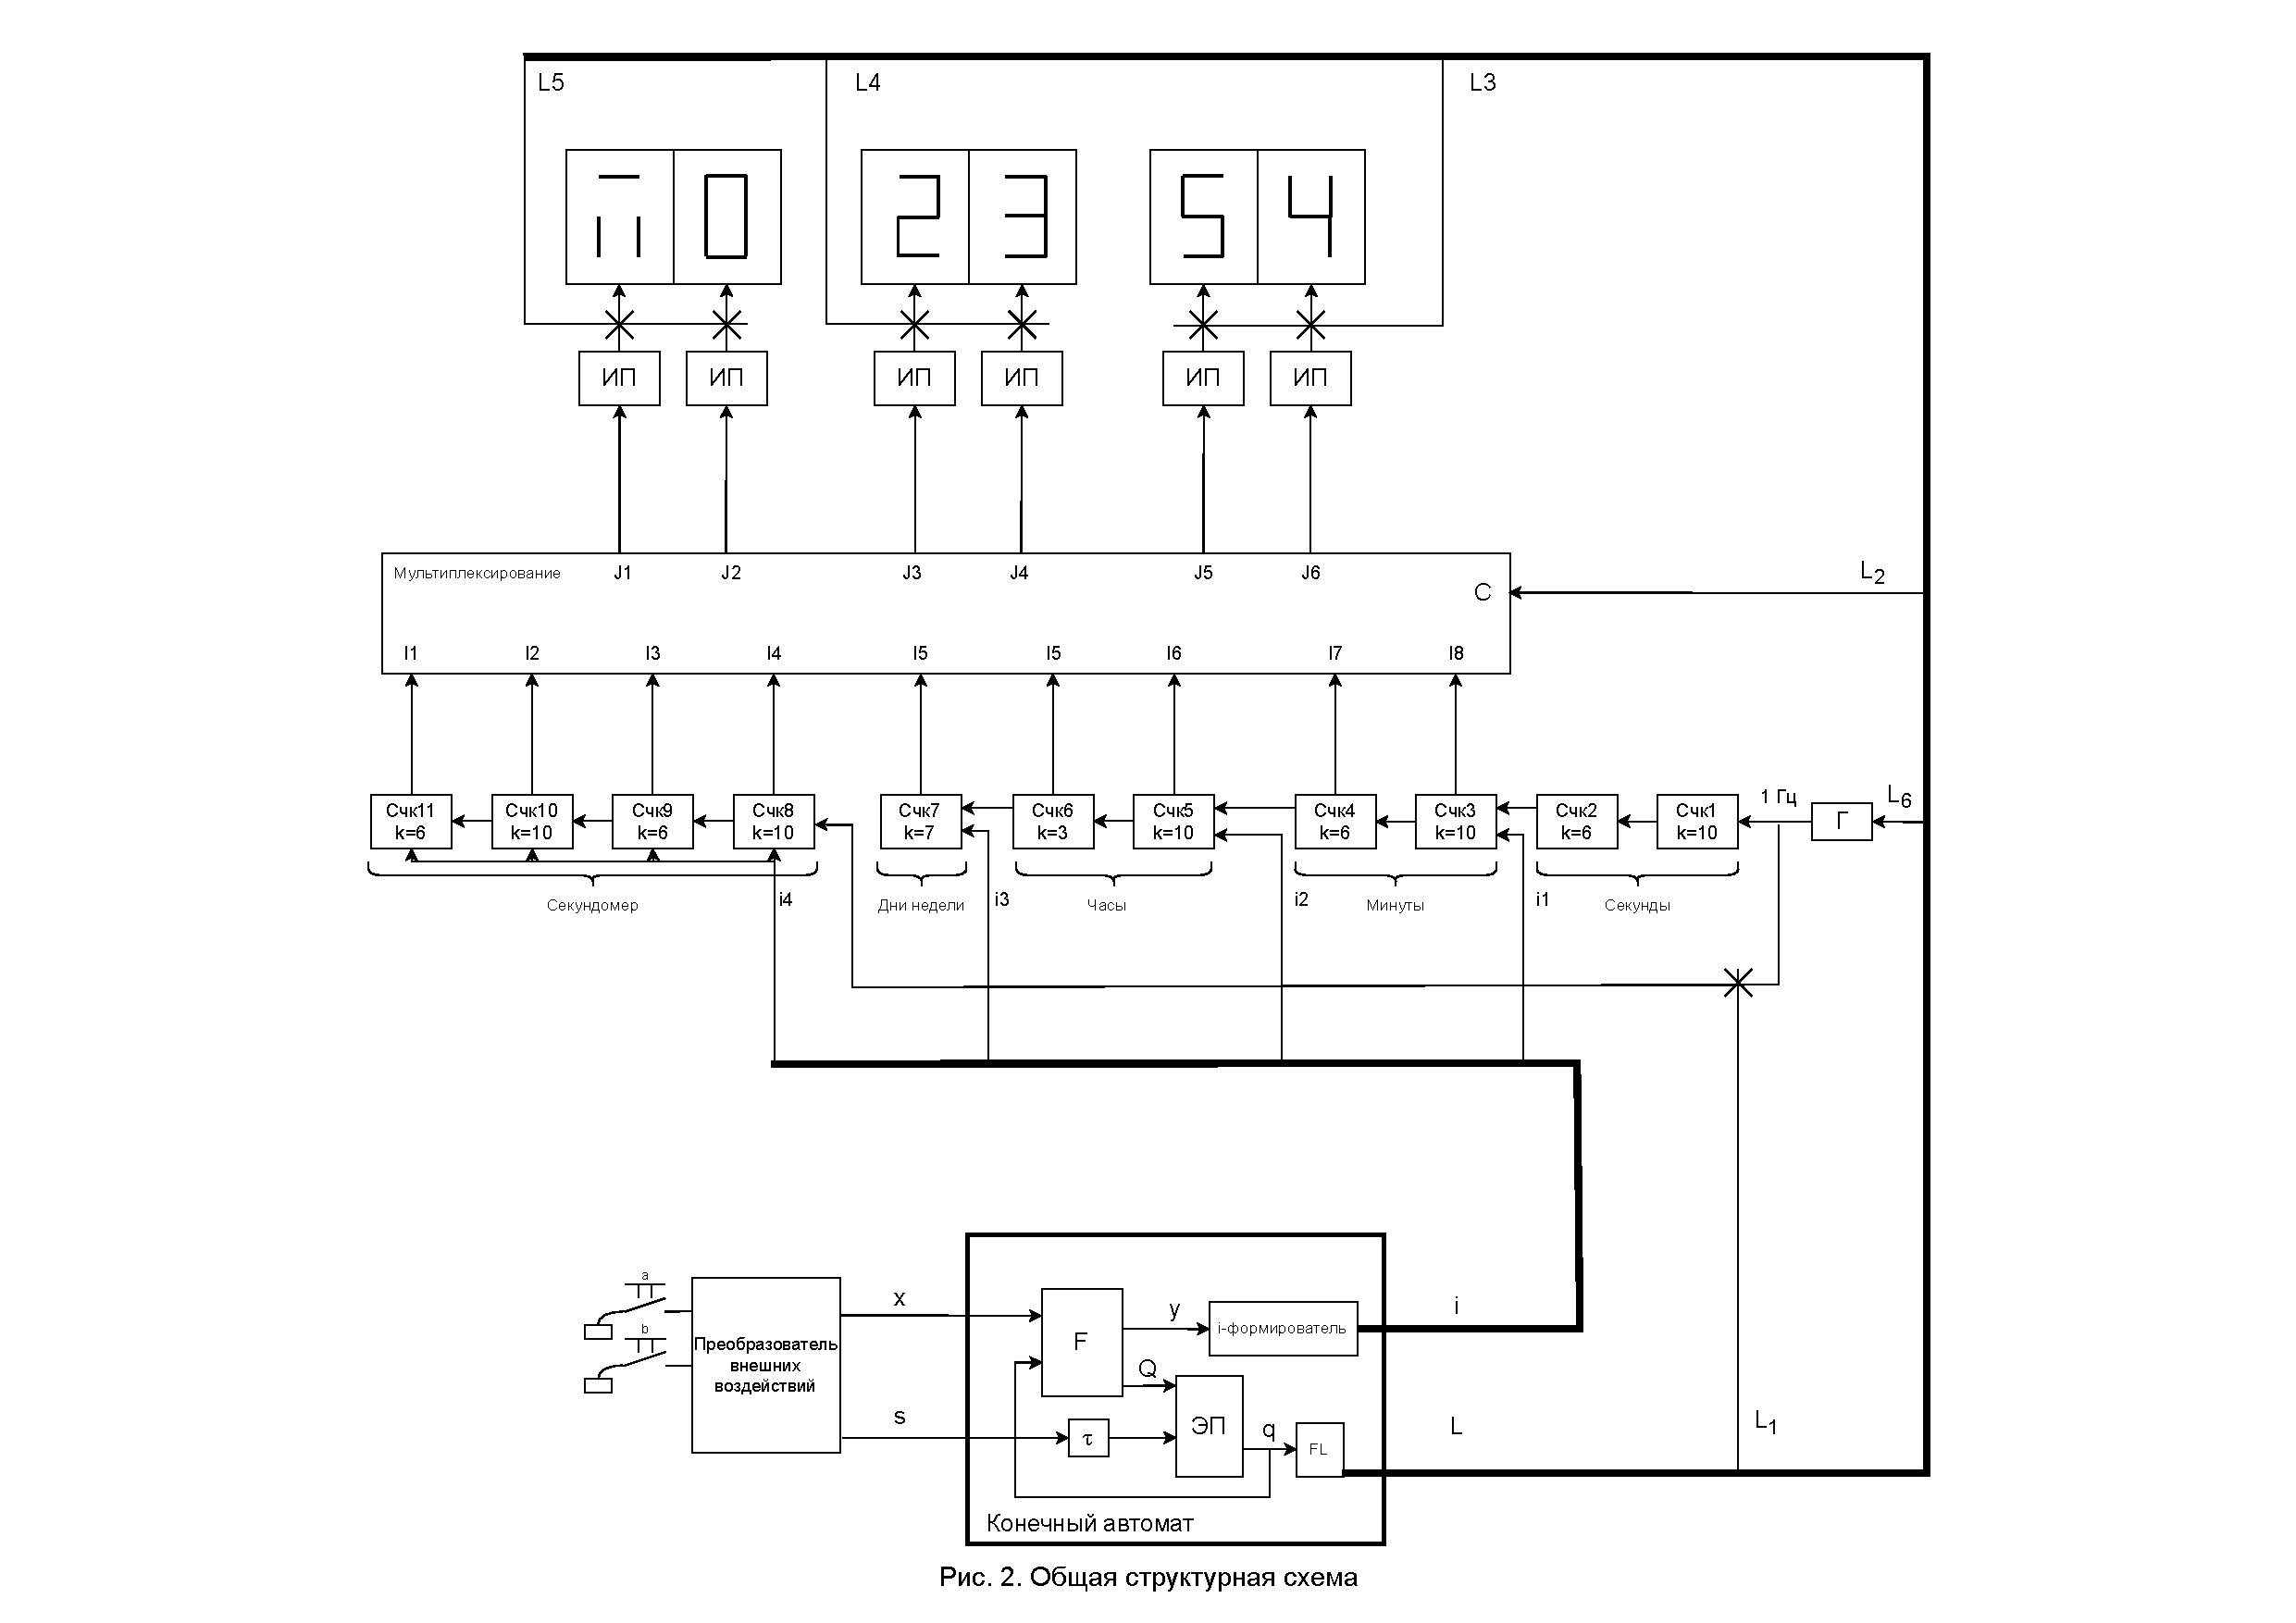
\includepdf[pages=1, fitpaper]{scheme.pdf}
\refstepcounter{figure}
\newpage

\subsection{Кодирование входных и выходных воздействий, состояний автомата}
Кодирование входных сигналов и состояний автомата представлены в Табл.~\ref{tbl:code_input} и Табл.~\ref{tbl:code_states} соответственно.

\begin{table}[h!]
  \centering
  \caption{Кодирование входных сигналов}
  \label{tbl:code_input}
  \footnotesize
  \begin{tabular}{|c|c|c|}
  \hline
        & $\mathbf{x_1}$& $\mathbf{x_2}$ \\
  \hline
  $\mathbf{a}$ & 1 & 0 \\
  \hline
  $\mathbf{b}$ & 0 & 1 \\
  \hline
  $\mathbf{ab}$ & 1 & 1 \\
  \hline
  \end{tabular}
\end{table}

\begin{table}[h!]
  \centering
  \caption{Кодирование состояний}
  \label{tbl:code_states}
  \footnotesize
  \begin{tabular}{|c|c|c|c|}
  \hline
        & $\mathbf{q_1}$& $\mathbf{q_2}$ & $\mathbf{q_3}$  \\
  \hline
  $\mathbf{S_0}$ & 0 & 0 & 0 \\
  \hline
  $\mathbf{S_1}$ & 0 & 0 & 1 \\
  \hline
  $\mathbf{S_2}$ & 0 & 1 & 0 \\
  \hline
  $\mathbf{S_3}$ & 0 & 1 & 1 \\
  \hline
  $\mathbf{S_4}$ & 1 & 0 & 0 \\
  \hline
  $\mathbf{S_5}$ & 1 & 0 & 1 \\
  \hline
  $\mathbf{S_6}$ & 1 & 1 & 0 \\
  \hline
  \end{tabular}
\end{table}


\subsection{Минимизация функций}
В соответствии с закодированными состояниями были построены таблицы истинности для преобразований F и FL (Табл.~\ref{tbl:f} и Табл.~\ref{tbl:fl}).

\begin{table}[h!]
  \centering
  \caption{Преобразование F}
  \label{tbl:f}
  \footnotesize

  \begin{tabularx}{\textwidth}{|c|c|X|X|X||X|X|X|c|c|c|c|}
  \hline
  \multicolumn{2}{|c|}{\textbf{Входы}} & \multicolumn{3}{c||}{\textbf{Текущее состояние}} & \multicolumn{3}{c|}{\textbf{Следующее состояние}} & \multicolumn{4}{c|}{\textbf{Выход}} \\
  \hline
  $\mathbf{x_1}$& $\mathbf{x_2}$ & $\mathbf{q_1}$ & $\mathbf{q_2}$ & $\mathbf{q_3}$ & $\mathbf{Q_1}$ & $\mathbf{Q_2}$ & $\mathbf{Q_3}$ & $\mathbf{i_1}$ & $\mathbf{i_2}$ & $\mathbf{i_3}$ & $\mathbf{i_4}$ \\
  \hline
  \hline
  %a/b/ab   S            S'           i1-i4
  %         S0
  1 & 0 &   0 & 0 & 0 &  0 & 0 & 1 &  0 & 0 & 0 & 0\\
  \hline
  0 & 1 &   0 & 0 & 0 &  1 & 0 & 0 &  0 & 0 & 0 & 0\\
  \hline
  1 & 1 &   0 & 0 & 0 &  1 & 1 & 0 &  0 & 0 & 0 & 0\\
  \hline

  %         S1
  1 & 0 &   0 & 0 & 1 &  0 & 1 & 0 &  0 & 0 & 0 & 0\\
  \hline
  0 & 1 &   0 & 0 & 1 &  0 & 0 & 1 &  1 & 0 & 0 & 0\\
  \hline
  1 & 1 &   0 & 0 & 1 &  0 & 0 & 1 &  0 & 0 & 0 & 0\\

  %         S2
  \hline
  1 & 0 &   0 & 1 & 0 &  0 & 1 & 1 &  0 & 0 & 0 & 0\\
  \hline
  0 & 1 &   0 & 1 & 0 &  0 & 1 & 0 &  0 & 1 & 0 & 0\\
  \hline
  1 & 1 &   0 & 1 & 0 &  0 & 1 & 0 &  0 & 0 & 0 & 0\\
  \hline
  
  %         S3
  1 & 0 &   0 & 1 & 1 &  0 & 0 & 0 &  0 & 0 & 0 & 0\\
  \hline
  0 & 1 &   0 & 1 & 1 &  0 & 1 & 1 &  0 & 0 & 1 & 0\\
  \hline
  1 & 1 &   0 & 1 & 1 &  0 & 1 & 1 &  0 & 0 & 0 & 0\\
  \hline

  %         S4
  1 & 0 &   1 & 0 & 0 &  1 & 0 & 0 &  0 & 0 & 0 & 0\\
  \hline
  0 & 1 &   1 & 0 & 0 &  1 & 0 & 1 &  0 & 0 & 0 & 0\\
  \hline
  1 & 1 &   1 & 0 & 0 &  0 & 0 & 0 &  0 & 0 & 0 & 0\\
  \hline

  %         S5
  1 & 0 &   1 & 0 & 1 &  1 & 0 & 1 &  0 & 0 & 0 & 1\\
  \hline
  0 & 1 &   1 & 0 & 1 &  1 & 0 & 0 &  0 & 0 & 0 & 0\\
  \hline
  1 & 1 &   1 & 0 & 1 &  0 & 0 & 0 &  0 & 0 & 0 & 0\\
  \hline

  %         S6
  1 & 0 &   1 & 1 & 0 &  1 & 1 & 0 &  0 & 0 & 0 & 0\\
  \hline
  0 & 1 &   1 & 1 & 0 &  1 & 1 & 0 &  0 & 0 & 0 & 0\\
  \hline
  1 & 1 &   1 & 1 & 0 &  0 & 0 & 0 &  0 & 0 & 0 & 0\\
  \hline
  \end{tabularx}
\end{table}

\begin{table}[h!]
  \centering
  \caption{Преобразование FL}
  \label{tbl:fl}
  \footnotesize
  \begin{tabular}{|c||c|c|c||c|c|c|c|c|c|}
  \hline
      & $\mathbf{q_1}$& $\mathbf{q_2}$ & $\mathbf{q_3}$ & $\mathbf{L_1}$ & $\mathbf{L_2}$ & $\mathbf{L_3}$ & $\mathbf{L_4}$ & $\mathbf{L_5}$ & $\mathbf{L_6}$ \\
  \hline
  \hline
  0   & 0 & 0 & 0   & 0 & 0 & 1 & 1 & 1 & 1 \\
  \hline
  1   & 0 & 0 & 1   & 0 & 0 & 1 & 0 & 0 & 1 \\
  \hline
  2   & 0 & 1 & 0   & 0 & 0 & 0 & 1 & 0 & 1 \\
  \hline
  3   & 0 & 1 & 1   & 0 & 0 & 0 & 0 & 1 & 1 \\
  \hline
  4   & 1 & 0 & 0   & 1 & 1 & 1 & 1 & 0 & 1 \\
  \hline
  5   & 1 & 0 & 1   & 0 & 1 & 1 & 1 & 0 & 1 \\
  \hline
  6   & 1 & 1 & 0   & 0 & 0 & 1 & 1 & 1 & 0 \\
  \hline
  \end{tabular}
\end{table}

\newpage
\subsubsection{Минимизация для $Q_1$-$Q_3$}
По Табл.~\ref{tbl:f} были построены формулы для $Q_1, Q_2, Q_3$. На Рис.~\ref{img:karno_q} приведены карты Карно для минимизации $Q_1, Q_2, Q_3$ соответственно.

\begin{figure}[H]
\centering \subfigure[]{
  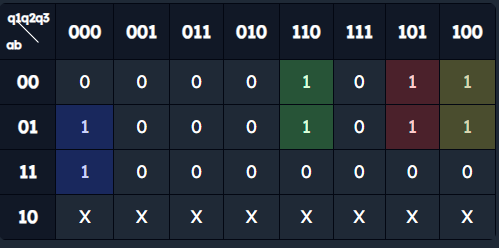
\includegraphics[width=0.4\linewidth]{q1.png} \label{img:q1} }  
  \hspace{4ex}
  \subfigure[]{
  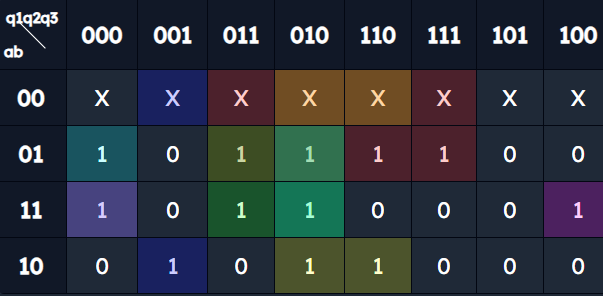
\includegraphics[width=0.4\linewidth]{q2.png} \label{img:q2} }
  \subfigure[]{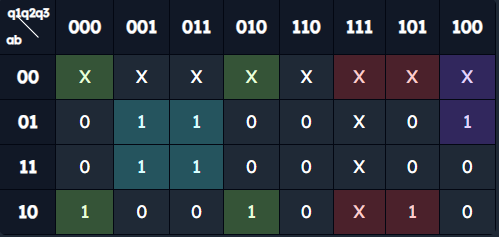
\includegraphics[width=0.4\linewidth]{q3.png} \label{img:q3} }  
  \caption{Карты карно для \subref{img:q1} $Q_1$; \subref{img:q2} $Q_2$;
  \subref{img:q3} $Q_3$.
  }
  \label{img:karno_q}
\end{figure}


\[Q_1 = \neg x_2 q_1 + \neg x_1 q_1 + x_2 \neg q_1 \neg q_2 \neg q_3\]
\[Q_2 = \neg x_1 q_2 + \neg x_2 q_2 \neg q_3 + x_2 q_2 q_3 + \neg x_2 \neg q_1 \neg q_2 q_3 + x_1 x_2 \neg q_1 \neg q_3\]
\[Q_3 = \neg x_2 q_1 q_3 + \neg x_2 \neg q_1 \neg q_3 + x_2 \neg q_1 q_3 + \neg x_1 q_1 \neg q_2 \neg q_3\]

\subsubsection{Минимизация для $i_1$-$i_4$}
По Табл.~\ref{tbl:f} были построены формулы для $i_1, i_2, i_3, i_4$. На Рис.~\ref{img:karno_i} приведены карты Карно для минимизации $i_1, i_2, i_3, i_4$ соответственно.

\begin{figure}[H]
  \centering \subfigure[]{
    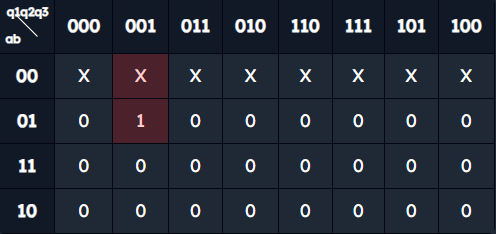
\includegraphics[width=0.4\linewidth]{i1.png} \label{img:i1} }  
    \hspace{4ex}
    \subfigure[]{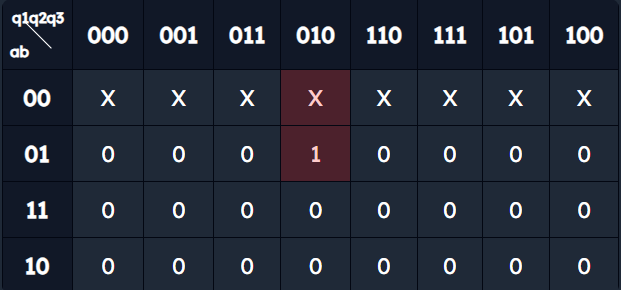
\includegraphics[width=0.4\linewidth]{i2.png} \label{img:i2} }
    \subfigure[]{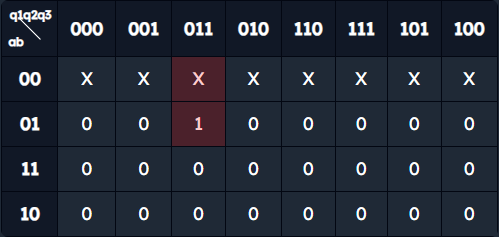
\includegraphics[width=0.4\linewidth]{i3.png} \label{img:i3} }  
    \hspace{4ex}
    \subfigure[]{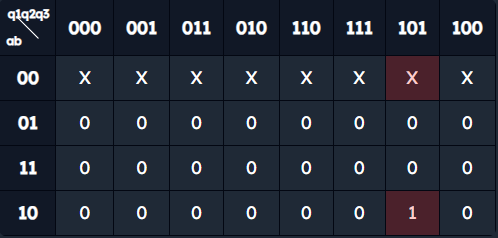
\includegraphics[width=0.4\linewidth]{i4.png} \label{img:i4} }
    \caption{Карты карно для \subref{img:i1} $i_1$; \subref{img:i2} $i_2$; \subref{img:i3} $i_3$; \subref{img:i4} $i_4$.
    }
    \label{img:karno_i}
  \end{figure}

\[i_1 = \neg x_1 \neg q_1 \neg q_2 q_3\]
\[i_2 = \neg x_1 \neg q_1 q_2 \neg q_3\]
\[i_3 = \neg x_1 q_2 q_3\]
\[i_4 = \neg x_2 q_1 q_3\]

\subsubsection{Минимизация для $L_1$-$L_6$}
По Табл.~\ref{tbl:fl} были построены формулы для $L_1, L_2, L_3, L_4, L_5, L_6$. На Рис.~\ref{img:karno_l} приведены карты Карно для минимизации $L_1, L_2, L_3, L_4, L_5, L_6$ соответственно.

\begin{figure}[H]
  \centering 
  \subfigure[]{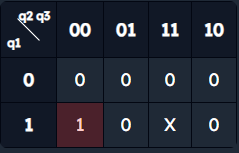
\includegraphics[width=0.4\linewidth]{l1.png} \label{img:l1} }  
  \hspace{4ex}
  \subfigure[]{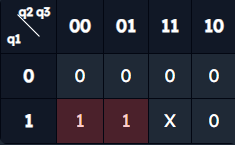
\includegraphics[width=0.4\linewidth]{l2.png} \label{img:l2} }
  \subfigure[]{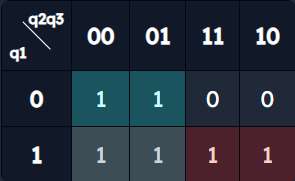
\includegraphics[width=0.4\linewidth]{l3.png} \label{img:l3} }  
  \hspace{4ex}
  \subfigure[]{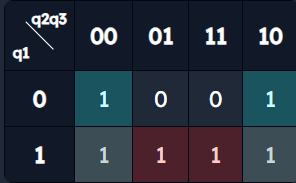
\includegraphics[width=0.4\linewidth]{l4.png} \label{img:l4} }
  \subfigure[]{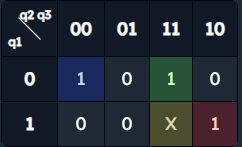
\includegraphics[width=0.4\linewidth]{l5.png} \label{img:l5} }  
  \hspace{4ex}
  \subfigure[]{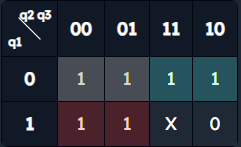
\includegraphics[width=0.4\linewidth]{l6.png} \label{img:l6} }
      
  \caption{Карты карно для \subref{img:l1} $L_1$; \subref{img:l2} $L_2$;
  \subref{img:l3} $L_3$; \subref{img:l4} $L_4$; \subref{img:l5} $L_5$;
  \subref{img:l6} $L_6$.
  }
  \label{img:karno_l}
  \end{figure}

\[L_1 = q_1 \neg q_2 \neg q_3\]
\[L_2 = q_1 \neg q_2\]
\[L_3 = q_1 + \neg q_2\]
\[L_4 = q_1 + \neg q_3\]
\[L_5 = q_1 q_2 + q_2 q_3 + \neg q_1 \neg q_2 \neg q_3\]
\[L_6 = \neg q_1 + \neg q_2\]

\newpage
\section{Схемотехническая реализация}
\subsection{Анализ схемотехнических элементов}
\subsubsection{Индикаторный преобразователь (ИП)}
\textit{Индикаторный преобразователь} (ИП) --- выполняет функцию преобразования двоичного кода, десятичной цифры в сигналы, которые управляют индикаторами. Каждый индикатор состоит из семи сегментов, коnjhst при включении в определенной комбинации формируют изображение соответствующей цифры. Необходимо подавать напряжение на каждый сегмент, чтобы он «загорелся» и отобразил нужную информацию. На Рис.~\ref{img:IC} приведены индикаторные преобразователи схемы.

\begin{figure}[H]
   \centering
   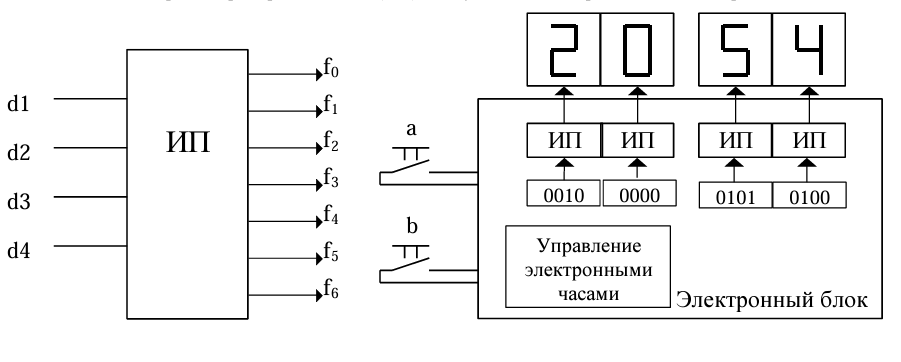
\includegraphics[width=1\linewidth]{IC.png}
   \caption{Индикаторный преобразователь}
   \label{img:IC}
\end{figure}

В данной работе был использован универсальный ИП 74LS47D, при помощи которого сигнал из четырёх бит, определяющий десятичную цифру, преобразовывался в соответствующие сигналы для отображения данной цифры на семисегментном дисплее.

\subsubsection{Тактовый генератор}
\textit{Генератор тактовых импульсов (генератор тактовой частоты)} предназначен для синхронизации различных процессов в цифровых устройствах --- ЭВМ, электронных часах, таймерах и других. Он вырабатывает электрические импульсы, обычно прямоугольной формы,
заданной частоты, которая часто используется как эталонная --- считая количество импульсов, можно, например, измерять временные интервалы. На Рис.~\ref{img:clock} показан тактовый генератор.

\begin{figure}[H]
   \centering
   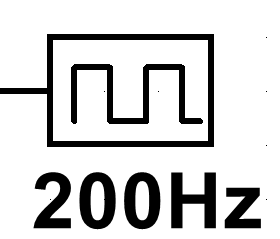
\includegraphics[scale=0.5]{clock.png}
   \caption{Тактовый генератор}
   \label{img:clock}
\end{figure}

В данной работе используется тактовый генератор с тактовой частотой 200 Гц, значением скважности 50\% и задержкой 0 секунд.

\subsubsection{Счётчик}
\textit{Счётчик} --- это устройство, которое осуществляет счет и хранение импульсов. У каждого счетчика есть тактовый вход, на который поступают импульсы, и несколько выходов, с которых можно снимать двоичный код числа, находящийся в счетчике. С каждым новым входным импульсом этот код изменяется: он может увеличиваться на 1 (суммирующий счетчик), уменьшаться на 1 (вычитающий счетчик) или изменяться в соответствии с каким-либо другим правилом. На Рис.~\ref{img:counters} приведена, работа двух счётчиков.

\begin{figure}[H]
   \centering
   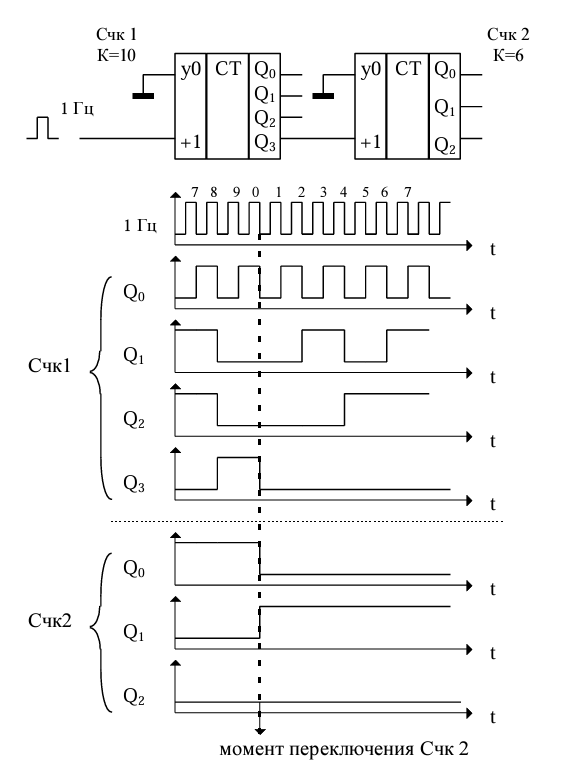
\includegraphics[width=0.5\linewidth]{counters.png}
   \caption{Работа счётчиков}
   \label{img:counters}
\end{figure}

Важным параметром счётчика является \textit{коэффициент пересчета} K. K --- это максимальное число импульсов, которое может быть подсчитано. Если рассматривать счетчик как конечный автомат, то K --- это количество различных состояний счетчика. Через K переключений счетчик c коэффициентом пересчета K возвращается в исходное состояние. Для удобства использования счетчика, кроме тактового входа существует вход «Уст. 0» (сброс). При подаче на него импульса (логической единицы) на выходе устанавливается нулевой код. 

\subsubsection{Триггер}
\textit{Триггер} --- устройство с двумя устойчивыми состояниями. Основная его функция --- хранить один бит информации неограниченное время до тех пор, пока эта информация не будет изменена воздействием на вход триггера. Существует довольно много разновидностей триггеров, различающихся по входным условиям смены состояния.

Кратко алгоритм работы D-триггера, используемого в дальнейшем (см. Рис.~\ref{img:trigger}): когда на выходе Q --- 1‚ а на выходе $\overline{\rm Q}$ --- 0, говорят, что триггер установлен в единичное состояние. В противном случае (Q --- 0, $\overline{\rm Q}$ --- 0), считается, что триггер сброшен в нулевое стояние. На выходе $\overline{\rm Q}$ триггера всегда устанавливается уровень напряжения, противоположный уровню напряжения на Q.

\begin{figure}[H]
   \centering
   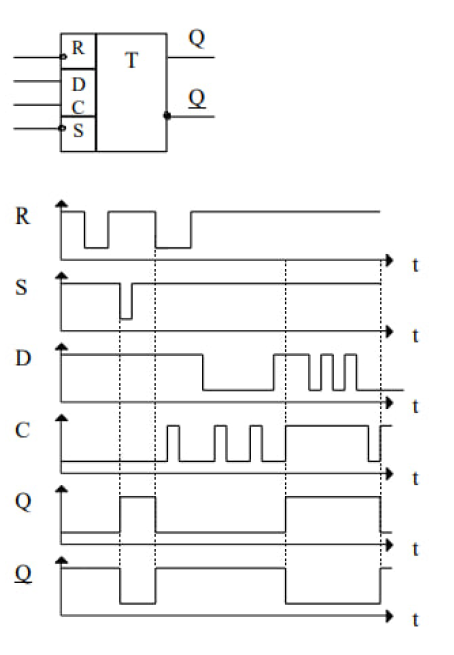
\includegraphics[scale=0.6]{trigger.png}
   \caption{D-триггер}
   \label{img:trigger}
\end{figure}

Непосредственная установка или сброс триггера осуществляется подачей напряжения низкого уровня на входы S (Set -- установка) или R (Reset -- сброс) соответственно. Подавать логический ноль на оба входа сразу недопустимо. Если низкий уровень присутствует на R или S, то сигналы на входах D и C никак не влияют на состояние триггера. Однако в функциональном плане более важными являются именно входы D (Data) и C (Clock). Триггер работает так, что сигнал от входа D передается на выход Q в момент положительного перепада напряжения на C. При этом во время постоянного уровня напряжения или в момент отрицательного перепада напряжения на C значение Q не может измениться. Чтобы триггер переключался правильно, уровень на входе D следует зафиксировать заранее, перед приходом тактового перепада на C. Минимальное время между появлением сигнала на D и на C называется защитным интервалом. При работе в таком режиме, на входах R и S должен присутствовать уровень логической единицы.

\cleardoublepage
\phantomsection
\newpage
\addcontentsline{toc}{section}{Заключение}
\section*{Заключение}


\cleardoublepage
\phantomsection
\newpage
%Список источников
\begin{thebibliography}{0}
	\bibitem{bib:algorithm}
	Теория алгоритмов [Электронный ресурс] URL: \url{https://tema.spbstu.ru/algorithm/} (дата обращения 10.12.2024).

  \bibitem{bib:sublime}
	sublime.tools. Карта карно [Электронный ресурс] URL: \url{https://sublime.tools/ru/karta-karno} (дата обращения 10.12.2024).
\end{thebibliography}
\addcontentsline{toc}{section}{Список источников}
\end{document}